\documentclass[a4paper,12pt]{article}
\usepackage[T1]{fontenc}
\usepackage[utf8]{inputenc}
\usepackage{mathtools}
\usepackage[italian]{babel}
%\usepackage{graphicx}
\usepackage{float}
\usepackage{textcomp}
\usepackage{amsmath}

\title{Esercitazione 1}
\author{Olivieri Daniele}
\date{}

\begin{document}
\maketitle
Valutare lo scambio di lavoro meccanico e di energia termica
delle seguenti trasformazioni:
\begin{itemize}
    \item Compressione adiabatica isoentropica di 1 kg di aria da
    1 bar e $288.15\ K$ a 2.5 bar.
    
    \item Compressione adiabatica reale di 1 kg di aria da 1 bar
    e 288.15 K a 2.5 bar con $\eta_{pc}$ pari a 0.755
   
    \item Compressione politropica di 1 kg di aria da 1 bar e 288.15 K a 2.5 bar
    con la condizione termodinamica finale coincidente con quella dell'adiabatica reale
   
    \item Compressione isoterma di 1 kg di aria da 1 bar e 288.15 K a 2.5 bar

    \item Compressione di 1 kg di acqua da 1 bar e 288.15 K a 2.5 bar
\end{itemize}

\section{Trasformazione isoentropica}
\label{sec:prima_trasformazione}
Analizziamo la prima trasformazione utilizzando le relazioni per le trasformazioni reversibili,
per prima cosa si determina lo stato del gas prima e dopo l'espansione mediante l'equazione
di stato dei gas
\begin{equation}
    \label{eq:stato_gas}
    pv = RT
\end{equation}
Lo stato iniziale è interamente determinato dato che conosciamo sia la temperatura che la pressione
mentre per il secondo dobbiamo utilizzare la politropica per trasformazioni reversibili,
in questo caso $x$ è proprio uguale a $k$, la costante del gas pari a $Cp/Cv$
\begin{equation}
    \label{eq:politropica}
    p\cdot v^x=\text{cost}
\end{equation}
Possiamo quindi ricavare $v_2$ tramite $$  v_2 = v_1/(\beta^{1/k}) $$

Determinato $v_2$ utilizzando ancora la \eqref{eq:stato_gas} calcoliamo il valore della temperatura
$T_2$ in uscita dal compressore.

Il lavoro necessario alla compressione sarà interamente speso per l'aumento di entalpia del gas
e potrà quindi essere calcolato con
\begin{equation}
    \label{eq:lavoro_isoentropico}
    L_{is} = m\cdot \Delta h = m\cdot C_p (T_2 - T_1)
\end{equation}
esso sarà pari a $86.65\ kJ$

Considerando la trasformazione adiabatica, il calore scambiato sarà nullo.

Tabella degli stati

\begin{center}
    \begin{tabular}{r|c|c|c}
        stato    & $p\ (bar)$ & $v\ (m^3/kg)$ & $T\ (\text{°}C) $\\ \hline
        1   &           1 &          0.827    &           15     \\ \hline
        2   &         2.5 &          0.429    &           101.2
    \end{tabular}
\end{center}

\section{Trasformazione adiabatica reale}
\label{sec:seconda_trasformazione}
Anche in questo caso la trasformazione è adiabatica ma viene fornito un valore del rendimento
politropico di compressione $\eta_{pc} = 0.755$, definito come
\begin{equation}
    \label{eq:rendimento_politropica}
    \eta_{pc} \stackrel{def}{=} \frac{\displaystyle\frac{n}{n-1} R T_1 \left(1-\beta^{\displaystyle\frac{n-1}{n}} \right)}{C_p \left(T_1 - T_2\right)}
    = \frac{L_{pc}}{L_r}
\end{equation}
o equivalentemente 
\begin{equation}
    \label{eq:rendimento_politropica_breve}
    \eta_{pc} = \frac{n}{n-1} \frac{k-1}{k}
\end{equation}
si può quindi ricavare il valore dell'esponente n della politropica oppure sostituire direttamente
il rendimento politropico nella definizione del rendimento adiabatico e quindi calcolarne il valore.
\begin{equation}
    \label{eq:rendimento_compressione_adiabatico}
    \eta_{ad_c} \stackrel{def}{=} \frac{L_{is}}{L_r} = \frac{ C_p T_1 \left(1-\beta^{\displaystyle\frac{k-1}{k}}\right)}
    {C_p T_1 \left(1-\beta^{\displaystyle\frac{n-1}{n}}\right)} = \frac{1-\beta^{\displaystyle\frac{k-1}{k}}}{1-\beta^{\displaystyle\frac{k-1}{k\eta_{pc}}}}
\end{equation}
svolgendo i calcoli si trova quindi un valore del rendimento adiabatico pari a $\eta_{ad_c}=0.722$.
Il lavoro necessario alla trasformazione adiabatica reale sarà quindi il rapporto tra il lavoro necessario
alla precedente trasformazione isoentropica e il rendimento adiabatico
\begin{equation*}
    L_r = \frac{L_{is}}{\eta_{ad_c}}
\end{equation*}
e sarà pari a $120\ kJ$.
Anche in questo caso il calore scambiato è considerato nullo.

\section{Trasformazione politropica}
\label{sec:terza_trasformazione}
La terza trasformazione richiede il calcolo delle condizioni termodinamiche dello stato finale della
compressione adiabatica reale, possiamo calcolare la politropica passante per gli stessi punti dato che
ci viene fornito il rendimento.
Riferendoci quindi alla \eqref{eq:politropica} dobbiamo calcolare il valore dell'esponente incognito
ricavabile dalla \eqref{eq:rendimento_politropica_breve} che sarà uguale a
\begin{equation}
    \label{eq:esp_politropica}
    n = \frac{\eta_{pc}}{\eta_{pc}-\displaystyle\frac{k-1}{k}}
\end{equation}
in questo caso pari a 1.609, maggiore del valore $k = 1.4$ per l'aria, com'era da aspettarsi.
Rieseguendo i calcoli svolti nella sezione \ref{sec:prima_trasformazione} possiamo creare la nuova tabella
degli stati termodinamici:

\begin{center}
    \begin{tabular}{r|c|c|c}
        stato    & $p\ (bar)$ & $v\ (m^3/kg)$ & $T\ (\text{°}C) $\\ \hline
        1   &           1 &          0.827    &           15     \\ \hline
        2   &         2.5 &          0.468    &           134.4
    \end{tabular}
\end{center}
temperatura e volume specifico sono maggiori rispetto alle condizioni successive alla trasforamzione
isoentropica.
Il lavoro necessario per la trasformazione politropica è ricavabile dalla definizione del rendimento politropico
\eqref{eq:rendimento_politropica} ed è pari a $90.6\ kJ$, per raggiungere lo stato termodinamico 2.
La differenza tra il lavoro reale e quello politropico è pari a $29.4\ kJ$ di energia che viene fornita al fluido
sotto forma di calore causato dagli attriti interni della macchina. Questa quantità è definita lavoro di contro-recupero.

\section{Trasformazione isoterma}
\label{sec:quarta_trasformazione}
La compressione isoterma implica una sottrazione di calore continua al fine di mantenere la temperatura
costante durante la compressione, tecnicamente irrealzzabile a causa della geometria dei compressori
fortemente adiabatici, si può ottenere invece una interrefrigerazione dividendo la compressione in più 
stadi.
Utilizzando ancora la \eqref{eq:politropica} e ponendo l'esponente pari ad 1 si ottiene l'equazione dell'isoterma
\begin{equation}
    p\cdot v = \text{cost}
\end{equation}
Ricaviamo quindi gli stati termodinamici come fatto in precedenza
\begin{center}
    \begin{tabular}{r|c|c|c}
        stato    & $p\ (bar)$ & $v\ (m^3/kg)$ & $T\ (\text{°}C) $\\ \hline
        1   &           1 &          0.827    &           15     \\ \hline
        2   &         2.5 &          0.331    &           15
    \end{tabular}
\end{center}
Il lavoro necessario alla compressione è pari al calore scambiato dal sistema dato che l'energia interna $U$
di un gas perfetto è funzione della sola temperatura, resta quindi anch'essa costante, ciò implica che
$Q = L$.
Il lavoro è facilmente calcolabile come 
\begin{equation}
    L = \int_{p_1}^{p_2} v\cdot dp
\end{equation}
utilizzando la \eqref{eq:stato_gas} e sostituendo $p$ si ricava:
\begin{equation}
    L = mRT\cdot \ln\beta
\end{equation}
Il lavoro di compressione isotermo è quindi pari a $75.8\ kJ$ così come anche il calore uscente necessario a 
mantenere la temperatura costante.

\section{Rendimenti}
Confronto tra i vari rendimenti delle trasformazioni appena viste.

Il rendimento adiabatico è stato definito nella \eqref{eq:rendimento_compressione_adiabatico} e il suo valore è di 0.722.

Il rendimento isotermo è invece così definito:
\begin{equation}
    \label{eq:rendimento_isotermo}
    \eta_{is_T} \stackrel{def}{=} \frac{L_{is_T}}{L_r}
\end{equation}
Il lavoro isotermo è stato calcolato nella sezione \ref{sec:quarta_trasformazione} e vale $75.8\ kJ$, il rendimento
vale quindi 0.632

L'esponente della politropica che passa per i punti della trasformazione reale è stato calcolato mediante 
la \eqref{eq:esp_politropica} e vale 1.609

\section{Compressione di un liquido}
\label{sec:compressione_liquido}
Valutare lo scambio di lavoro meccanico ed energia termica necessari alla compressione di 1 kg di acqua da
1 bar e $288.15 K$ a 2.5 bar.
Nell'ipotesi di processo adiabatico reversibile, il lavoro necessario sarà pari all'integrale 
\begin{equation}
    L = \int_{p_1}^{p_2} v\cdot dp
\end{equation}
considerato inoltre il modello di liquido ideale, il volume specifico si può assumere costante, rendendo banale
il calcolo dell'integrale, tenendo in considerazione il fatto che la pressione va espressa in Pascal
per una corretta analisi dimensionale.
\begin{equation}
    L = mv(p_2-p_1)
\end{equation}
Sarà pari a $150\ J$.

\section{Valutazioni complessive}
\label{sec:valutazioni_complessive}
Mediante l'ausilio del software GeoGebra sono state rappresentate le trasformazioni compiute dall'aria negli esempi
precedenti nel piano T-s.
\begin{figure}[H]
    \label{fig:trasformazioni}
    \centering
    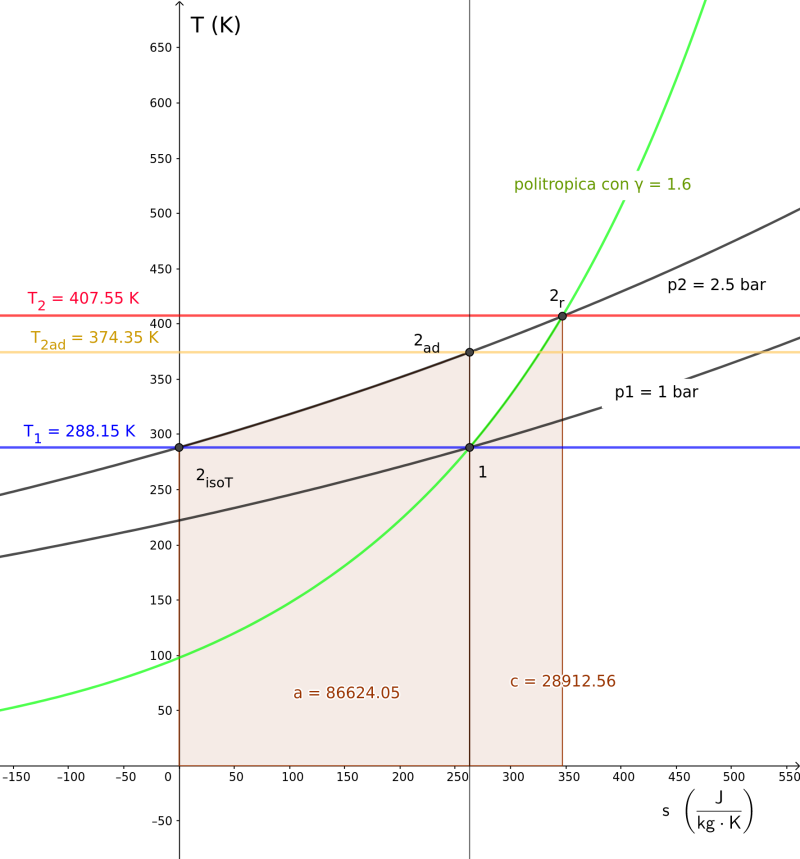
\includegraphics[width=0.65\linewidth]{media/isobare_T-S_resize.png}
    %\caption{"Etichetta"}
\end{figure}
Per prima cosa sono stati impostati i valori di temperatura iniziale e finale dalle tabelle, tracciando le isoterme
$T_1\ T_2$ e $T_{2ad}$ e fissata arbitrariamente (per semplicità di calcolo) entropia nulla allo stato $2_{isoT}$.
Utilizzando la relazione dell'entropia in forma integrale per trasformazioni isoterme
\begin{equation*}
    \Delta s = R\ln\beta
\end{equation*}
sono state misurate la variazioni di entropia specifica per la trasformazione isoterma e quindi la coordinata x dello stato iniziale 1
pari a $263\ J/(kg\cdot K)$.
\subsection{Rappresentazione delle isobare}
Per rappresentare le isobare nel piano T-s è stato sufficiente sfruttare l'equazione dell'entropia per gas perfetti,
semplificando il termine contenente il rapporto tra le pressioni. Gli stati termodinamici presi in considerazione
per imporre il passaggio delle curve sono quello iniziale (1) e quello successivo alla trasformazione isoterma ($2_{isoT}$)
in questo modo il valore iniziale $T_0$ è lo stesso per entrambe le isobare.
Svolgendo i passaggi:
\begin{gather*}
    \Delta s = C_p \ln \frac{T}{T_0} \\
    \frac{s - s_0}{C_p} = \ln\frac{T}{T_0} \\
    T = T_0 \exp \frac{s-s_0}{C_p}
\end{gather*}
con $T_0$ pari a 288.15 ed $s_0$ pari a 0 per la isobara a pressione maggiore e 263 per quella passante per il punto iniziale.
Intersecando l'isobara maggiore con la isoterma $T_2$ è stato possibile individuare il punto $2_r$ successivo alla compressione reale
e valutarne l'entropia.

\subsection{Rappresentazione della politropica}
Facendo riferimento alla \eqref{eq:politropica} ed avendo calcolato l'esponente tramite la \eqref{eq:esp_politropica}
utilizzando il rendimento fornito dall'esercizio, è stato possibile scrivere rappresentare la trasformazione sul piano T-s
imponendo il passaggio per i punti 1 e $2_r$
% \begin{equation*}
%     p v^k = \text{cost}
% \end{equation*}
% per rappresentarla nel piano T-s sono stati necessari però alcuni passaggi:
\begin{gather*}
    pv^k = \text{cost} \\
    kpv^{k-1}dv + v^kdp = 0
\end{gather*}
raccogliendo e semplificando per $v^{k-1}$ si ottiene
\begin{equation}
    \label{eq:politropica_differenziata}
    kpdv + vdp = 0
\end{equation}   
differenziando invece la \eqref{eq:stato_gas} e sostituendo il termine $vdp$ nella \eqref{eq:politropica_differenziata}
si ottiene:
\begin{gather*}
    (k-1)pdv + RdT = 0 \\
    pdv = -\frac{RdT}{k-1}
\end{gather*}
sostituendo anche in questo caso nell'equazione dell'entropia (questa volta in forma differenziale)
si ottiene:
\begin{gather*}
    Tds = C_vdT -\frac{R}{k-1}dT \\
    \frac{dT}{T} = \frac{k-1}{C_v(k-1)-R} ds
\end{gather*}
integrando
\begin{equation*}
    \ln\frac{T}{T_0} = \frac{k-1}{C_v(k-1)-R}\cdot(s-s_0)
\end{equation*}
l'equazione della politropica sarà dunque
\begin{equation}
    T = T_0 \exp\left(\frac{k-1}{C_v(k-1)-R}\cdot(s-s_0)\right)
\end{equation}
con k pari a 1.6, il termine $(s-s_0)$ va diviso per 1000 dato che la scala dell' entropia è espressa in J
e non in kJ.
Si può vedere che la curva della politropica ottenuta interseca la isoterma superiore e
l'isobara nello stesso punto.

\subsection{Valutazione dei lavori}
Per sistemi aperti adiabatici il lavoro è pari alla variazione di entalpia del fluido, nel caso
di gas perfetti è pari a $C_p(\Delta T)$ ed è definito $C_p$ la quantità di calore da fornire
per innalzare di 1 grado la temperatura di una massa unitaria di gas in una trasformazione isobara.

Per il secondo principio
\begin{equation}
    \label{eq:seconmdo_principio}
    Tds = dq + dl
\end{equation}
il lavoro necessario alla trasformazioni adiabatica isoentropica sarà per questo motivo l'area sottesa
alla isobara isobara $p_2$ dal punto $2_{isoT}$ ad entropia nulla al punto $2_{ad}$
mentre quello necessario alla trasformazione adiabatica reale si otterrà eseguendo lo stesso integrale tra i punti
$2_{isoT}$ e $2_r$.
La differenza tra questi due valori è pari al lavoro valutabile mediante l'integrale della politropica tra i punti
1 e $2_r$ sommato al lavoro di contro-recupero.

Mediante la funzione "Integrale" definita in GeoGebra è possibile valutare facilmente
l'area sottesa alle funzioni appena rappresentate.
% Eseguendo l'integrale della isobara $p_2$ dal punto $2_{isoT}$ ad entropia nulla al punto $2_{ad}$
% si ottiene il lavoro della compressione adiabatica isoentropica, eseguendo l'integrale della stessa funzione
% dal punto $2_{isoT}$ al punto $2_r$ si ottiene invece il lavoro necessario alla trasformazione adiabatica reale.

\section{Confronto livelli di energia}
Confrontare i livelli di energia meccanica scambiata nelle precedenti trasformazioni con 
quella potenziale posseduta da un uomo di peso medio (80 kg) che si trovi ad una quota di 150 m.
La variazione di energia potenziale gravitazionale è facilmente ricavabile tramite la relazione
\begin{equation}
    \Delta U = mg\Delta h
\end{equation}
% \textit rende il testo corsivo

dove
\begin{itemize}
    \item[\textit{m}] è la massa del corpo (kg)
    \item[\textit{g}] è l'accelerazione gravitazionale terrestre pari a 9.81 $(m/s^2)$ 
    \item[\textit{h}] è l'altezza in metri
\end{itemize}  
Fissato il valore dell'energia nullo al livello del mare, una massa di 80 kg a 150 m avrà
un'energia potenziale gravitazionale di 117.72 kJ.

Confrontiamo ora in una tabella i valori di queste energie scambiate
\begin{center}
    \begin{tabular}{l|c}
        Trasformazione & Energia scambiata (kJ)\\ \hline
        Compressione reale        & 120  \\
        Compressione politropica  & 90.6 \\
        Compressione isoentropica & 86.5 \\
        Compressione isoterma     & 75.8 \\
        Compressione liquido      & 150$\cdot 10^{-3}$  \\
        Uomo che scala 150 m      & 117.2
    \end{tabular}
\end{center}

\section{Rendimento compressori commerciali}
Calcolare il rendimento politropico $\eta_{pc}$ di un compressore avente
\begin{itemize}
    \item[$\beta$] = 30
    \item[$\eta_{ad_c}$] = 0.86
\end{itemize}
Facendo riferimento alla \eqref{eq:rendimento_compressione_adiabatico} si ricava per prima cosa il valore
del coefficiente \textit{n} tramite alcuni passaggi
% \begin{equation}
%     n = \frac{-1}{\frac{\ln\left(\frac{\eta_{ad}-1+\beta^{\frac{k-1}{k}}}{\eta_{ad}}\right)}{\ln\beta}-1}
% \end{equation}
\begin{equation}
    n = \frac{\ln\beta}{\ln\beta - \ln\left(\frac{\eta_{ad}-1+\beta^{\frac{k-1}{k}}}{\eta_{ad}}\right)}
\end{equation}
e vale in questo caso 1.46.
Si può quindi ricavare il rendimento politropico dalla \eqref{eq:rendimento_politropica_breve} che vale in questo caso 0.91.

Analizziamo ora la targa di un compressore commerciale da officina, reperita dal produttore \textit{CECCATO}
\begin{figure}[H]
    \centering
    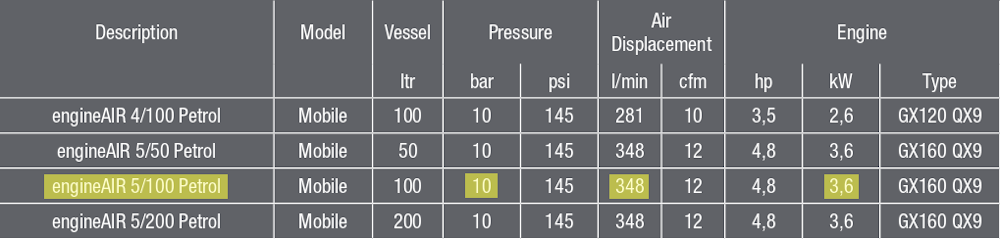
\includegraphics[width=0.99\linewidth]{media/catalogo.png}
\end{figure}
scelto il modello \textit{engineAIR 5/100 Petrol} i valori di nostro interesse sono:

\begin{itemize}
    \item [\textit{Pressione:}] il valore di massima pressione in uscita al compressore
    \item[\textit{Portata d'aria:}] quantità d'aria aspirata in l/min 
    \item[\textit{Potenza motore:}] potenza massima erogabile dal motore
\end{itemize} 

Dato che non possediamo la curva di andamento pressione/potenza non possiamo stimare il rendimento se non nella condizione
di massimo regime, ossia ad una pressione in uscita pari a 10 bar ed una potenza di 3.6 kW.
Per prima cosa fissiamo le condizioni ambientali di aspirazione ad 1 bar e 25°C, in questo modo utilizzando il modello
di gas ideale e ricavato il volume specifico possiamo valutare la portata massica, più comoda per i calcoli.
Se la portata volumetrica è espressa in l/min, per trasformarla in kg/s dobbiamo effettuare la seguente conversione:
\begin{equation*}
    \dot{m} = \frac{\dot{V}}{v}
\end{equation*}
dove \textit{v} è il volume specifico del gas e $\dot{V}$ è espressa in $m^3/s$, da l/min a $m^3/s$ bisogna dividere per 60000.

Rieseguendo i passaggi svolti nella sezione \ref{sec:prima_trasformazione} si ottiene la tabella degli stati ideali
\begin{center}
    \begin{tabular}{r|c|c|c}
        stato    & $p\ (bar)$ & $v\ (m^3/kg)$ & $T\ (\text{°}C) $\\ \hline
        1   &           1 &          0.856    &           25     \\ \hline
        2   &          10 &          0.165    &           302
    \end{tabular}
\end{center}
e dopo aver valutato la potenza meccanica necessaria alla trasformazione isoentropica mediante la \eqref{eq:lavoro_isoentropico}
si può facilmente valutare il rendimento adiabatico di compressione definito nella \eqref{eq:rendimento_compressione_adiabatico}
e pari a 0.525.

Ottenuto il rapporto di compressione e il rendimento adiabatico, ripetendo i passaggi svolti per il compressore fornito dall'esercizio
si può ottenere il rendimento politropico pari a 0.645.
Ricavato il valore dell'esponente della politropica con la \eqref{eq:esp_politropica} si può determinare lo stato reale in uscita dal compressore.
\begin{center}
    \begin{tabular}{r|c|c|c}
        stato    & $p\ (bar)$ & $v\ (m^3/kg)$ & $T\ (\text{°}C) $\\ \hline
        1   &           1 &          0.856    &           25     \\ \hline
        2   &          10 &          0.237    &           554
    \end{tabular}
\end{center}
I rendimenti del secondo compressore, volumetrico monostadio, sono di gran lunga inferiori rispetto ad un compressore assiale (dinamico) multistadio.
\end{document}
